% Options for packages loaded elsewhere
\PassOptionsToPackage{unicode}{hyperref}
\PassOptionsToPackage{hyphens}{url}
\PassOptionsToPackage{dvipsnames,svgnames,x11names}{xcolor}
%
\documentclass[
  letterpaper,
  DIV=11,
  numbers=noendperiod]{scrartcl}

\usepackage{amsmath,amssymb}
\usepackage{iftex}
\ifPDFTeX
  \usepackage[T1]{fontenc}
  \usepackage[utf8]{inputenc}
  \usepackage{textcomp} % provide euro and other symbols
\else % if luatex or xetex
  \usepackage{unicode-math}
  \defaultfontfeatures{Scale=MatchLowercase}
  \defaultfontfeatures[\rmfamily]{Ligatures=TeX,Scale=1}
\fi
\usepackage{lmodern}
\ifPDFTeX\else  
    % xetex/luatex font selection
\fi
% Use upquote if available, for straight quotes in verbatim environments
\IfFileExists{upquote.sty}{\usepackage{upquote}}{}
\IfFileExists{microtype.sty}{% use microtype if available
  \usepackage[]{microtype}
  \UseMicrotypeSet[protrusion]{basicmath} % disable protrusion for tt fonts
}{}
\makeatletter
\@ifundefined{KOMAClassName}{% if non-KOMA class
  \IfFileExists{parskip.sty}{%
    \usepackage{parskip}
  }{% else
    \setlength{\parindent}{0pt}
    \setlength{\parskip}{6pt plus 2pt minus 1pt}}
}{% if KOMA class
  \KOMAoptions{parskip=half}}
\makeatother
\usepackage{xcolor}
\setlength{\emergencystretch}{3em} % prevent overfull lines
\setcounter{secnumdepth}{-\maxdimen} % remove section numbering
% Make \paragraph and \subparagraph free-standing
\makeatletter
\ifx\paragraph\undefined\else
  \let\oldparagraph\paragraph
  \renewcommand{\paragraph}{
    \@ifstar
      \xxxParagraphStar
      \xxxParagraphNoStar
  }
  \newcommand{\xxxParagraphStar}[1]{\oldparagraph*{#1}\mbox{}}
  \newcommand{\xxxParagraphNoStar}[1]{\oldparagraph{#1}\mbox{}}
\fi
\ifx\subparagraph\undefined\else
  \let\oldsubparagraph\subparagraph
  \renewcommand{\subparagraph}{
    \@ifstar
      \xxxSubParagraphStar
      \xxxSubParagraphNoStar
  }
  \newcommand{\xxxSubParagraphStar}[1]{\oldsubparagraph*{#1}\mbox{}}
  \newcommand{\xxxSubParagraphNoStar}[1]{\oldsubparagraph{#1}\mbox{}}
\fi
\makeatother


\providecommand{\tightlist}{%
  \setlength{\itemsep}{0pt}\setlength{\parskip}{0pt}}\usepackage{longtable,booktabs,array}
\usepackage{calc} % for calculating minipage widths
% Correct order of tables after \paragraph or \subparagraph
\usepackage{etoolbox}
\makeatletter
\patchcmd\longtable{\par}{\if@noskipsec\mbox{}\fi\par}{}{}
\makeatother
% Allow footnotes in longtable head/foot
\IfFileExists{footnotehyper.sty}{\usepackage{footnotehyper}}{\usepackage{footnote}}
\makesavenoteenv{longtable}
\usepackage{graphicx}
\makeatletter
\newsavebox\pandoc@box
\newcommand*\pandocbounded[1]{% scales image to fit in text height/width
  \sbox\pandoc@box{#1}%
  \Gscale@div\@tempa{\textheight}{\dimexpr\ht\pandoc@box+\dp\pandoc@box\relax}%
  \Gscale@div\@tempb{\linewidth}{\wd\pandoc@box}%
  \ifdim\@tempb\p@<\@tempa\p@\let\@tempa\@tempb\fi% select the smaller of both
  \ifdim\@tempa\p@<\p@\scalebox{\@tempa}{\usebox\pandoc@box}%
  \else\usebox{\pandoc@box}%
  \fi%
}
% Set default figure placement to htbp
\def\fps@figure{htbp}
\makeatother

\usepackage{booktabs}
\usepackage{longtable}
\usepackage{array}
\usepackage{multirow}
\usepackage{wrapfig}
\usepackage{float}
\usepackage{colortbl}
\usepackage{pdflscape}
\usepackage{tabu}
\usepackage{threeparttable}
\usepackage{threeparttablex}
\usepackage[normalem]{ulem}
\usepackage{makecell}
\usepackage{xcolor}
\usepackage{tabularray}
\usepackage[normalem]{ulem}
\usepackage{graphicx}
\UseTblrLibrary{booktabs}
\UseTblrLibrary{rotating}
\UseTblrLibrary{siunitx}
\NewTableCommand{\tinytableDefineColor}[3]{\definecolor{#1}{#2}{#3}}
\newcommand{\tinytableTabularrayUnderline}[1]{\underline{#1}}
\newcommand{\tinytableTabularrayStrikeout}[1]{\sout{#1}}
\KOMAoption{captions}{tableheading}
\usepackage{float}
\floatplacement{table}{H}
\makeatletter
\@ifpackageloaded{caption}{}{\usepackage{caption}}
\AtBeginDocument{%
\ifdefined\contentsname
  \renewcommand*\contentsname{Table of contents}
\else
  \newcommand\contentsname{Table of contents}
\fi
\ifdefined\listfigurename
  \renewcommand*\listfigurename{List of Figures}
\else
  \newcommand\listfigurename{List of Figures}
\fi
\ifdefined\listtablename
  \renewcommand*\listtablename{List of Tables}
\else
  \newcommand\listtablename{List of Tables}
\fi
\ifdefined\figurename
  \renewcommand*\figurename{Figure}
\else
  \newcommand\figurename{Figure}
\fi
\ifdefined\tablename
  \renewcommand*\tablename{Table}
\else
  \newcommand\tablename{Table}
\fi
}
\@ifpackageloaded{float}{}{\usepackage{float}}
\floatstyle{ruled}
\@ifundefined{c@chapter}{\newfloat{codelisting}{h}{lop}}{\newfloat{codelisting}{h}{lop}[chapter]}
\floatname{codelisting}{Listing}
\newcommand*\listoflistings{\listof{codelisting}{List of Listings}}
\makeatother
\makeatletter
\makeatother
\makeatletter
\@ifpackageloaded{caption}{}{\usepackage{caption}}
\@ifpackageloaded{subcaption}{}{\usepackage{subcaption}}
\makeatother

\usepackage{bookmark}

\IfFileExists{xurl.sty}{\usepackage{xurl}}{} % add URL line breaks if available
\urlstyle{same} % disable monospaced font for URLs
\hypersetup{
  pdftitle={Homework 5},
  pdfauthor={Ethan Murakami},
  colorlinks=true,
  linkcolor={blue},
  filecolor={Maroon},
  citecolor={Blue},
  urlcolor={Blue},
  pdfcreator={LaTeX via pandoc}}


\title{Homework 5}
\usepackage{etoolbox}
\makeatletter
\providecommand{\subtitle}[1]{% add subtitle to \maketitle
  \apptocmd{\@title}{\par {\large #1 \par}}{}{}
}
\makeatother
\subtitle{ECON 470, Spring 2025}
\author{Ethan Murakami}
\date{}

\begin{document}
\maketitle


Here is a link to my repository: \{https://github.com/bemur3/hwk5\}

\newpage

\newpage

\subsection{1. Plot the share of the adult population with direct
purchase health insurance over
time.}\label{plot-the-share-of-the-adult-population-with-direct-purchase-health-insurance-over-time.}

\pandocbounded{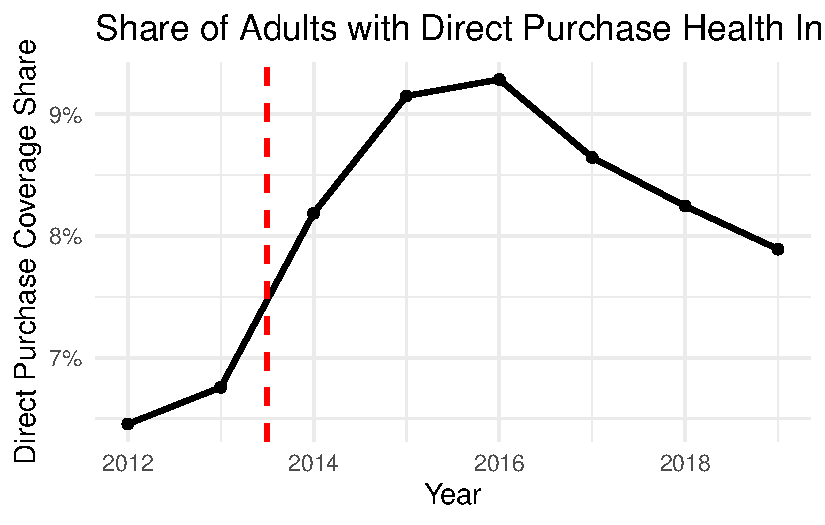
\includegraphics[keepaspectratio]{hwk5_files/figure-pdf/unnamed-chunk-3-1.pdf}}

\newpage

\subsection{2. Discuss the reduction in direct purchase health insurance
in later years. Can you list a couple of policies that might have
affected the success of the direct purchase insurance
market?}\label{discuss-the-reduction-in-direct-purchase-health-insurance-in-later-years.-can-you-list-a-couple-of-policies-that-might-have-affected-the-success-of-the-direct-purchase-insurance-market}

\newpage

\subsection{3. Plot the share of the adult population with Medicaid over
time}\label{plot-the-share-of-the-adult-population-with-medicaid-over-time}

\pandocbounded{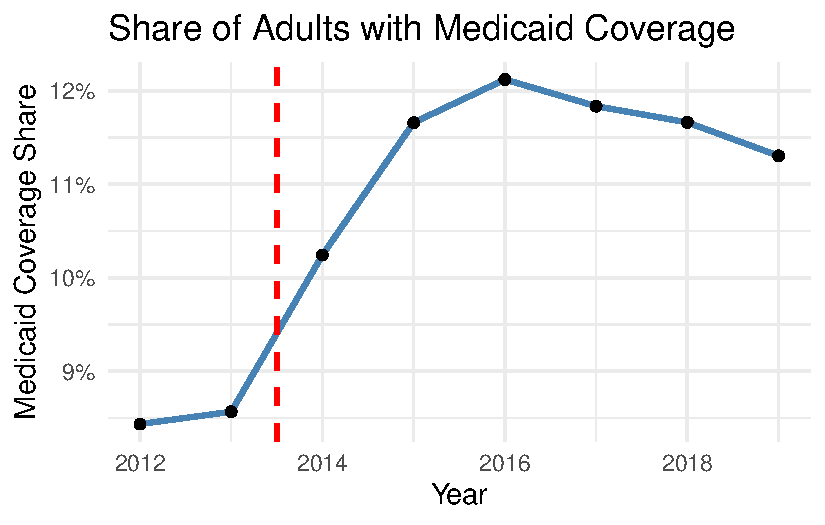
\includegraphics[keepaspectratio]{hwk5_files/figure-pdf/unnamed-chunk-4-1.pdf}}

\newpage

\subsection{4. Plot the share of uninsured over time, separately by
states that expanded Medicaid in 2014 versus those that did not. Drop
all states that expanded after
2014.}\label{plot-the-share-of-uninsured-over-time-separately-by-states-that-expanded-medicaid-in-2014-versus-those-that-did-not.-drop-all-states-that-expanded-after-2014.}

\pandocbounded{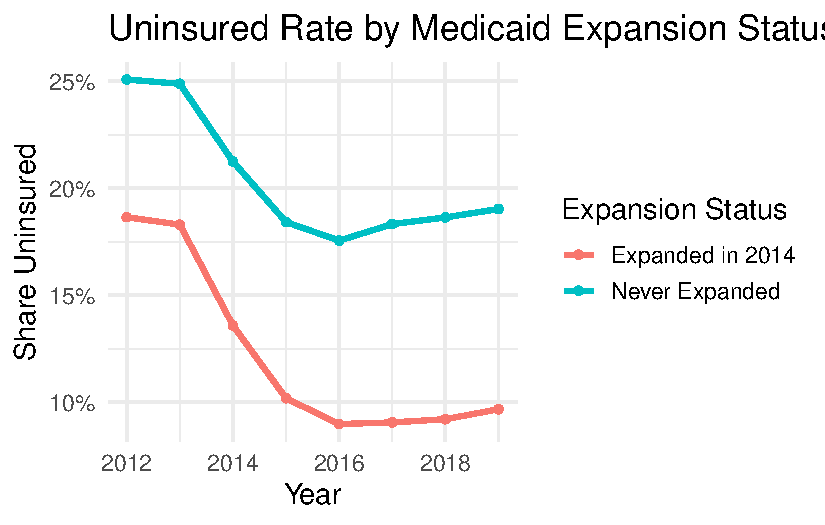
\includegraphics[keepaspectratio]{hwk5_files/figure-pdf/unnamed-chunk-5-1.pdf}}

\newpage

\subsection{5. Calculate the average percent of uninsured individuals in
2012 and 2015, separately for expansion and non-expansion states.
Present your results in a basic 2x2 DD
table.}\label{calculate-the-average-percent-of-uninsured-individuals-in-2012-and-2015-separately-for-expansion-and-non-expansion-states.-present-your-results-in-a-basic-2x2-dd-table.}

\begin{table}
\centering
\caption{DD Table for Medicaid Expansion}
\centering
\begin{tabular}[t]{lrr}
\toprule
Group & Pre & Post\\
\midrule
Expanded in 2014 & 0.17 & 0.09\\
Never Expanded & 0.21 & 0.16\\
\bottomrule
\end{tabular}
\end{table}

\newpage

\subsection{6. Estimate the effect of Medicaid expansion on the
uninsurance rate using a standard DD regression estimator, again
focusing only on states that expanded in 2014 versus those that never
expanded.}\label{estimate-the-effect-of-medicaid-expansion-on-the-uninsurance-rate-using-a-standard-dd-regression-estimator-again-focusing-only-on-states-that-expanded-in-2014-versus-those-that-never-expanded.}

\begin{table}
\centering
\begin{talltblr}[         %% tabularray outer open
caption={Standard DD Estimates for Medicaid Expansion},
]                     %% tabularray outer close
{                     %% tabularray inner open
colspec={Q[]Q[]},
column{2}={}{halign=c,},
column{1}={}{halign=l,},
hline{10}={1,2}{solid, black, 0.05em},
}                     %% tabularray inner close
\toprule
& (1) \\ \midrule %% TinyTableHeader
(Intercept) & \num{0.211} \\
& (\num{0.009}) \\
Post 2014 & \num{-0.052} \\
& (\num{0.011}) \\
Expand & \num{-0.044} \\
& (\num{0.011}) \\
Post x Expand & \num{-0.021} \\
& (\num{0.013}) \\
Num.Obs. & \num{304} \\
R2 & \num{0.455} \\
RMSE & \num{0.04} \\
\bottomrule
\end{talltblr}
\end{table}

\newpage

\subsection{7. Include state and year fixed effects in your estimates.
Try using the lfe or fixest package to estimate this instead of directly
including the fixed
effects.}\label{include-state-and-year-fixed-effects-in-your-estimates.-try-using-the-lfe-or-fixest-package-to-estimate-this-instead-of-directly-including-the-fixed-effects.}

\begin{table}
\centering
\begin{talltblr}[         %% tabularray outer open
caption={DD Estimates: Standard vs TWFE},
]                     %% tabularray outer close
{                     %% tabularray inner open
colspec={Q[]Q[]Q[]},
column{2,3}={}{halign=c,},
column{1}={}{halign=l,},
hline{10}={1,2,3}{solid, black, 0.05em},
}                     %% tabularray inner close
\toprule
& Standard DD & TWFE \\ \midrule %% TinyTableHeader
(Intercept) & \num{0.211} &  \\
& (\num{0.009}) &  \\
Post 2014 & \num{-0.052} &  \\
& (\num{0.011}) &  \\
Expand & \num{-0.044} &  \\
& (\num{0.011}) &  \\
Post x Expand & \num{-0.021} & \num{-0.021} \\
& (\num{0.013}) & (\num{0.009}) \\
Num.Obs. & \num{304} & \num{304} \\
R2 & \num{0.455} & \num{0.944} \\
R2 Within &  & \num{0.082} \\
RMSE & \num{0.04} & \num{0.01} \\
Std.Errors &  & by: State \\
\bottomrule
\end{talltblr}
\end{table}

\newpage

\subsection{8. Repeat the analysis in question 7 but include all states
(even those that expanded after 2014). Are your results different? If
so,
why?}\label{repeat-the-analysis-in-question-7-but-include-all-states-even-those-that-expanded-after-2014.-are-your-results-different-if-so-why}

\begin{table}
\centering
\begin{talltblr}[         %% tabularray outer open
caption={DD Estimates: Including Staggered Expansions},
]                     %% tabularray outer close
{                     %% tabularray inner open
colspec={Q[]Q[]Q[]Q[]},
column{2,3,4}={}{halign=c,},
column{1}={}{halign=l,},
hline{12}={1,2,3,4}{solid, black, 0.05em},
}                     %% tabularray inner close
\toprule
& Standard DD & TWFE & Time-varying Treatment \\ \midrule %% TinyTableHeader
(Intercept) & \num{0.211} &  &  \\
& (\num{0.009}) &  &  \\
Post 2014 & \num{-0.052} &  &  \\
& (\num{0.011}) &  &  \\
Expand & \num{-0.044} &  &  \\
& (\num{0.011}) &  &  \\
Post x Expand & \num{-0.021} & \num{-0.021} &  \\
& (\num{0.013}) & (\num{0.009}) &  \\
Post x Expand (Dynamic) &  &  & \num{-0.024} \\
&  &  & (\num{0.006}) \\
Num.Obs. & \num{304} & \num{304} & \num{416} \\
R2 & \num{0.455} & \num{0.944} & \num{0.946} \\
R2 Within &  & \num{0.082} & \num{0.156} \\
RMSE & \num{0.04} & \num{0.01} & \num{0.01} \\
Std.Errors &  & by: State & by: State \\
\bottomrule
\end{talltblr}
\end{table}

\newpage

\subsection{9. Provide an ``event study'' graph showing the effects of
Medicaid expansion in each year. Use the specification that includes
state and year fixed effects, limited to states that expanded in 2014 or
never
expanded.}\label{provide-an-event-study-graph-showing-the-effects-of-medicaid-expansion-in-each-year.-use-the-specification-that-includes-state-and-year-fixed-effects-limited-to-states-that-expanded-in-2014-or-never-expanded.}

\pandocbounded{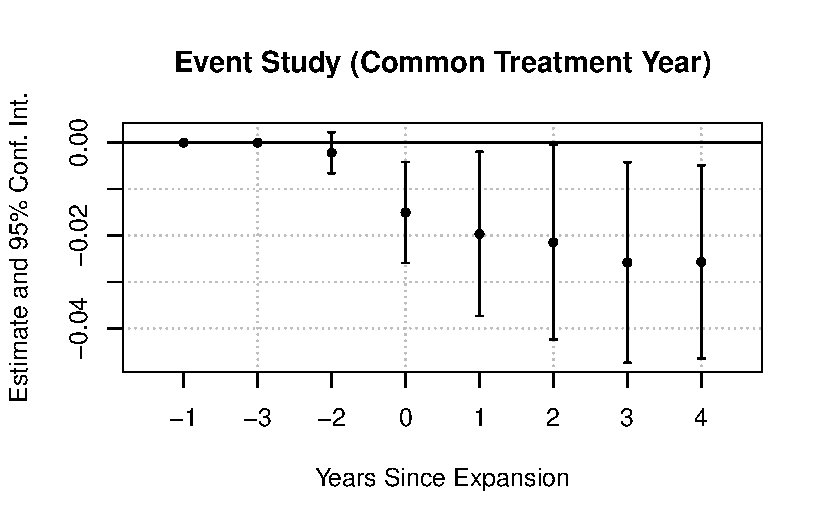
\includegraphics[keepaspectratio]{hwk5_files/figure-pdf/unnamed-chunk-10-1.pdf}}

\newpage

\subsection{10.Repeat part 9 but again include states that expanded
after 2014. Note: this is tricky\ldots you need to put all states onto
``event time'' to create this
graph.}\label{repeat-part-9-but-again-include-states-that-expanded-after-2014.-note-this-is-trickyyou-need-to-put-all-states-onto-event-time-to-create-this-graph.}

\pandocbounded{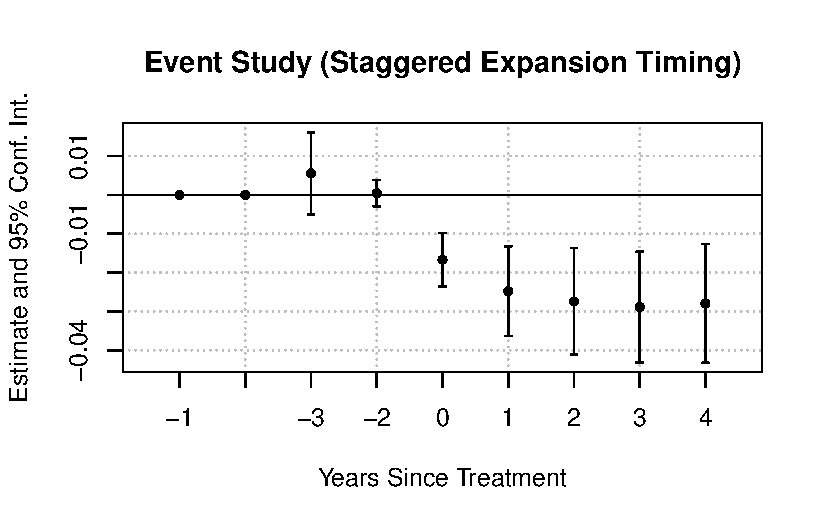
\includegraphics[keepaspectratio]{hwk5_files/figure-pdf/unnamed-chunk-11-1.pdf}}

\begin{verbatim}
NULL
\end{verbatim}




\end{document}
